\section{Loop-Freedom}
\label{sec:loop-free}

\subsection{Example}
\label{sec:example}

\begin{figure}[t!]
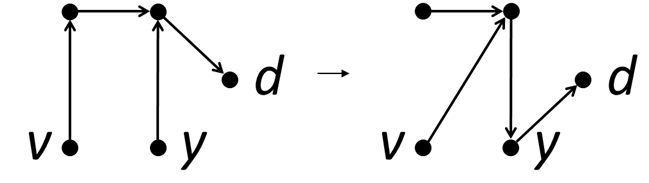
\includegraphics[width=3in]{figures/noloops.png}
\caption{Running example, discussed in Section \ref{sec:example}.}
\label{fig:example}
\end{figure}

Applying routing updates in a way that guarantees no loops is a basic but already interesting consistency property. Consider the five node example network with a single destination $d$ in Figure \ref{fig:example}. The existing routing to destination $d$ on the left of the figure should be updated according to the right of the figure. A naive way to update is to simply send out the forwarding updates (e.g., ``node $u$: for destination $d$ send to $x$''). However, when doing so, it might happen that node $x$ updates its rule before node $y$, introducing a routing loop between nodes $x$ and $y$. This loop will eventually disappear, namely once node $y$ updates its rule, but in an asynchronous system it is difficult to give guarantees when this will happen.

At the other end of the spectrum, the SDN controller could first (i) distribute the new rules, then (ii) wait for an acknowledgement of all the nodes that they have received the new rules, then (iii) tell all the nodes to stop sending packets, and finally, once (iv) they all acknowledged that, (v) tell the nodes to now use the new rules. After the nodes (vi) acknowledge that they are using the new rules, the SDN controller can tell them to (vii) remove the old rules, as they are not needed anymore. This solution does not suffer from loops, as the old and the new solution are well-separated in time.\footnote{Strictly speaking, this protocol is not sufficient, as there might be packets in transit, still using the old rules when rushing through the protocol. Consider a packet sent from sent from $y$ to $x$ shortly before $y$ received the order to stop sending (iii). If node $x$ already passed the last step of the protocol when receiving the packet, node $x$ has not other option then sending the packet back to node $y$, i.e. the packet is experiencing a loop.} However, it is also terribly slow. One may speed up the process by omitting steps (iii) and (iv). Now, assuming that node $x$ received the command to use the new rule (v) earlier than node $y$. As such, in order to guarantee no loop between nodes $x$ and $y$, we must introduce version numbers in packets such that nodes $x$ and $y$ know that packets from $x$ respectively $y$ must be treated according to the new respectively old rules. This is the solution proposed by \ref{theoriginalprincetonpaper}.

One may ask whether version numbers are really necessary, just to guarantee no loops? Also, one may ask whether a faster solution is possible. What nodes are really dependent on each other? This may look like a technicality, but as we all know, nodes are often temporarily unavailable or reacting slowly. If a node must wait for another node, there should better be a consistency reason for it, and not merely protocol overhead. Is there something like a \emph{minimal protocol for a given consistency guarantee}? This is exactly the question we address in this paper.

Regarding our example, the answer to this question is quite simple. Node $u$ does not even need to change its rule, as it always just forwards to $x$, hence node $u$ does not even have to be informed about the rule changes. Node $v$ can switch immediately after being informed about the new rule, as no matter whether using the old or new rule, the packet will always end up at node $x$, with no possibility to experience a loop. Also node $y$ can switch immediately to the new rule, as its packet will then directly reach the destination node $d$. The only critical node in our example is node $x$, for which we understand that node $x$ must wait until node $y$ implemented the switch, as otherwise our network might experience a loop.

More generally, achieving loop-free consistency requires rule updates to wait for each other in a \emph{dependency tree}, i.e., a node may have to wait for one parent node having switched to the new rule before being able to switch itself. Let the destination $d$ be the root of the dependency tree.

We will show two solutions, one with advantages regarding practice as the parent in the dependency forest is always a neighbor node. The practical solution is provably fast, however, it is not optimal regarding dependencies. So, in addition, we also show a more theoretical solution, which (in polynomial time) can compute the minimal dependency forest, i.e. where nodes can switch to the new solution in minimal time.
A node $p$ is a parent of a child node $c$ in the dependency forest if $c$ points to $p$ according to the new rules, e.g. $x$ is a parent of $u$ and $v$. Now, starting at the root, nodes first switch to the new rule, and then inform all their children in the dependency tree to switch as well. Apart from the packets-in-transit problem described above, correctness is immediate: Nodes that are in the dependency tree of the destination will only switch to the new rule once all the nodes on the new path to the destination have already switched. Based on the discussion on the example, it is easy to see that this solution is not minimal, as node $v$ cannot switch immediately, after learning the new rule, but must wait on $x$.

\begin{figure}[t!]
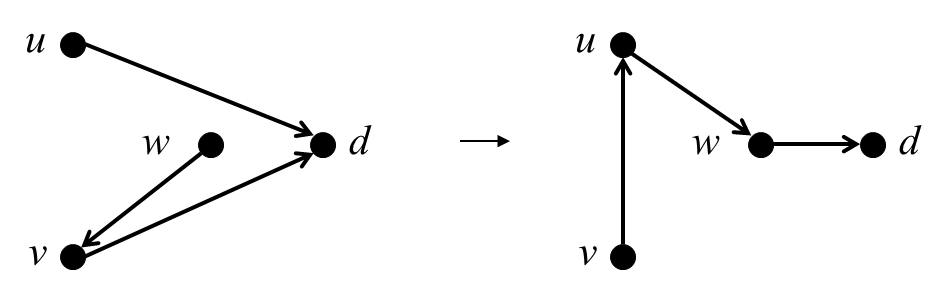
\includegraphics[width=3in]{figures/nominimum.png}
\caption{Example with two orthogonal minimal solutions, discussed in Section \ref{sec:minimal}.}
\label{fig:minimal}
\end{figure}

One may wish for a protocol which is as fast as possible, in the sense that dependencies are minimum. Quite
surprisingly, in general this is not trivial. Consider the four node example network in Figure \ref{fig:minimal}, again with the old rules on the left, and the new rules on the right. Node $w$ may switch to the new rule immediately. However, nodes $u$ and $v$ may not. If they both switch to the new rule immediately, and $w$ is still using the old rule, we introduced a loop. So one of them must wait for $w$ having switched. However, either one is fine, i.e. either $u$ must wait for $w$ (and $v,w$ may switch immediately), \emph{or} $v$ must wait for $w$ (and $u,w$ may switch immediately). If we switch the rules of node $u$ in the example in Figure \ref{fig:minimal}, such that \texttt{u.old = w} and \texttt{u.new = d}, we have another interesting case: Now, in order to prevent a loop, node $v$ must wait, but node $v$ may wait for either node $u$ \emph{or} node $w$. These examples show that optimality is a non-trivial concept that deserves further research.

\subsection{Minimal Protocol}
\label{sec:minimal}

Instead, in the following, we will present a protocol which is \emph{minimal} regarding its dependencies, in the sense that no node can improve its dependencies without some other node getting worse. As the example in Figure \ref{fig:example} shows, often there may be many nodes that can switch immediately, for different reasons. As such the dependency tree turns into a \emph{dependency forest}. As before, in this dependency forest, parents will inform their children when it is safe to use the new rule. The only difference is that the dependency forest is minimal, in the sense that one cannot remove a subtree of the forest with subtree root $c$ (and parent $p$) and re-attach it at a parent of $p$, or make $c$ a root of the forest. For simplicity, we first describe the protocol as if there was just a single destination $d$. We later discuss the case where we have multiple destinations.

Each node is in one of three states, \emph{old}, \emph{new}, or \emph{limbo}, depending on whether the node is guaranteed to only use its old rule or new rule, or whether it might use both rules, respectively. Since the destination $d$ does not have any rules, neither old nor new, it is by definition new.

The algorithm constructs the dependency forest as follows: We start out with only the old rules, by definition a loop-free in-tree to destination $d$. Now, for each node $u$, we test whether adding $u$'s new rule will introduce a loop. If not, node $u$ is entering the state limbo, and added as a root in the dependency forest. On the other hand, if $u$'s new rule introduces a loop, node $u$ remains old, and must wait until we find its parent in the dependency forest. The initialization is completed after we found all the roots (which are now leaves in the dependency forest). Next we add the children to the dependency forest, one after another. In each step, we choose a limbo dependency forest leaf node $u$. We remove $u$'s old rule from the network (putting $u$ in the new state), and then cycle through all the old nodes, trying to find nodes $v$ where the new rule of $v$ does not introduce a loop, thanks to removing $u$'s old rule. If we find such a node $v$, then node $v$ is a child of $u$ in the dependency forest, and a new leaf of the dependency forest in limbo state. If no such node $v$ exists, node $u$ remains a childless leaf of the dependency forest. It may happen that we find no more limbo node, that is, all nodes are either new or old. In this case, as proved below in Lemma 3 (TODO), we will always find an old node that can become new directly. 
We continue until we processed all nodes in the network.

At the heart of this algorithm is the simple loop-finder of Tarjan \cite{reference_1_in_http://en.wikipedia.org/wiki/Tarjan's_strongly_connected_components_algorithm} which can be implemented linearly in the size of the network. Since we must process each node, and check for each not yet processed node, the total time of the algorithm is cubic in the size of the network. We suspect that this running time can be improved, but this is beyond the scope of this paper. Clearly, the order in which the nodes are visited will determine the dependency forest, however, we will guarantee that no matter what the order is, the dependency tree is minimal.

TODO: alternative formulation, shorter, maybe better: Initially, we let all good nodes to be roots of the dependency forest. Then, iteratively, while not all nodes are processed, we process an arbitrary good node $u$ by removing its old rule. Removing $u$'s old rule might turn other nodes good; if $v$ turns good when processing $u$, then $v$ is a child of $u$ in the dependency forest.

TODO: explain Tarjan in simple terms.

\subsection{Proofs} %TODO: should probably not be a subsection, just did that for navigability.

In the following, we prove a few simple lemmas, which show that (i) the dependency forest is correct and (ii) minimal in the sense that if any node switches to the new rule before the parent in the dependency forest says so, a packet might be experiencing a loop.

Lemma 1: The invariant of the algorithm is that the current rules in the network is without loops.

Proof: This invariant is true at the beginning, since no new rule is included, and the old rules form an in-tree to the destination $d$. This invariant remains true when a node enters the limbo state (uses both old and new rules) as we check at this stage that no loop is introduced when doing so. Finally, the statement is true as well when a node enters the new state: As this only removes an old rule, no loop can be introduced.

Lemma 2: The dependency forest is loop-free. 

Proof: As the parent of a child must be in the dependency forest already, there cannot be loops in the dependency forest.

Lemma 3: At the end, every node (but the destination $d$) is in the dependency forest.

Proof: As long as there are nodes in limbo state, we will move them to the new state, one after the other, possibly moving other nodes from old to limbo. What if no node remains in limbo state, i.e. all nodes are either new or old. Then, as the algorithm suggests, there is always at least one node which can directly jump from old state to new state. We can find this node as follows: Start from an arbitrary old node, and move along the new rules towards the destination $d$. Since the destination is (by definition) new, along this new-rules path, there must be a last pair of nodes $c,p$, where \texttt{c.new = p}, $c$ and $p$ are old and new, respectively. Node $c$ can directly move to state new, $c$'s parent in the dependency forest is $p$. Removing $c$'s old rule will not introduce a loop, as removing a rule never introduces new loops. Also, adding $c$'s new rule does not introduce a loop, as it points to nodes which are in the new state already, that is, there are no more old rules which can cause loops. 

Remark: There are networks where this jumping mechanism is necessary. Example: A network with three nodes, where \texttt{u.old = v}, \texttt{u.new = d}, \texttt{v.old = d}, and \texttt{v.new = u}. Either of the nodes $u,v$ cannot enter the limbo state, as will be a loop between $u$ and $v$. 

Lemma 4: The process is correct (and produces no loops).

Proof: The follows directly from the dependency tree, as we only added nodes once they did not introduce a loop (Lemma 1).

Lemma 5: The process is minimal.

Proof: Root nodes in the dependency forest can flip to the new rule immediately, and are as such by definition optimal. A node $c$ is a child of a parent node $p$ in the dependency tree, exactly because $c$ can only use its new rule after $p$ removed its old rule. As such, the process guaranteed that $c$ was added to the dependency tree at the earliest possible time.

\subsection{Discussion} %TODO: should probably not be a subsection, just did that for navigability.

Let us now discuss some of the issues and additional features of this minimal dependency forest. First, what happens if the network is in the middle of a transition, and the SDN controller decides to update some rules (that might or might not have been rolled out already)? This can be integrated easily in the algorithm described above. In a nutshell, we just need to consider all rules that are possibly still existing in the network as old rules. As such, a node $u$ may have several old rules, pointing to different neighbors, plus one new rule. The definition of good/bad nodes then includes all these old rules. If some old rules have already been deleted, or have not been initiated, they can be ignored. Since our algorithm also works in the presence of a whole set of old rules, it can automatically handle updates that interrupt transitions.

A main cause for interrupting updates may be failures at nodes or edges. Essentially, failures may be handled in a standard way, by simply rolling out another batch of rules that will fix the failures. However, there is one exception, which we will first describe with an example: If some link $l$ is considered to be down, new rules will be introduced that route around this failed link $l$. An old rule on link $l$ might have a loop with some of the new rules, and as such the algorithm cannot push the new rules before the old rule is removed. Even worse, if the node $u$ holding the old rule is not accessible, the algorithm will not be able to push the fixing rules before node $u$ is reachable again. The SDN controller has a conflict of interest, it needs to quickly push a fix which must ignore (delete) the old rule, however, if unreachable node $u$ comes up again while doing so, the existing old rule will introduce a loop. (TODO: must be re-written, I just wanted to describe the problem.)

It is generally debatable whether SDN controllers are the best way to quickly handle errors. Going through the SDN controller always introduces some extra lag, after detecting an error. One may want to consider additional distributed ways to fix an error quickly, e.g. techniques such as link reversal \cite{originallinkreversalpaperforinstanceorsomethingnewer}

One other question is regarding time, in particular, how bad is the worst-case updates. Consider a $n$-node network with a ring topology. In the old regime, all nodes point clockwise to destination $d$. In the new regime, all nodes point counter-clockwise to destination $d$. Let us call clockwise neighbor of $d$ node $u_1$, the clockwise neighbor of $u_i$ is node $u_{i+1}$. In other words, the counter-clockwise neighbor of $d$ is node $u_{n-1}$. In this example, the dependency forest is a linked list $u_1,u_2,\ldots,u_{n-1}$, in other words, if the dependency forest is synchronized with a SDN controller, no matter where in the ring network the SDN controller is located, $\Theta(n^2)$ messages are going to be exchanged before the network adopted the new solution. This is the worst example, as the dependency forest cannot be worse than a linked list.

One other major question is what if we update several routes to several (or even all) destinations at the same time. A new rule at a node $u$ may be responsible for a whole prefix $p$ of destinations. In this case, optimality/minimality may be defined in different ways, as some sub-prefixes of prefix $p$ at node $u$ may be good earlier than others. For example, it may be that prefix $p0$ will be good immediately, as it remains unchanged, whereas prefix $p1$ will end up in a loop if we switch immediately. One may now say that the new rule for prefix $p$ should be split up into two rules $p0$ and $p1$, making it possible to switch at least $p0$ immediately. Then the solution above is straight-forward, as we just split up the addressing space into all the minimal sub-prefixes, computing dependency forests for all of them independently. However, even though this solution is in some sense time-minimal, it may be space-inefficient since new rules may now be split up into many sub-prefix rules.

Instead, we may want to define minimality with the original new rules in mind, that is, the new rule of node $u$ for prefix $p$ should not be used before it is loop-free. The concern is that this might lead to deadlocks or sub-optimal time bounds. Indeed, if rules are bundled to meta-rules arbitrarily, one might end up with a deadlock. The canonical example is a triangle network with three nodes and destinations $u,v,w$. The old routing is always clockwise, for two hops. The new routing is counter-clockwise, also for two hops. In other words, in both the old and the new solution, on each of the three links, two destinations are bundled into one rule. Now, no matter which is the three rules is initiated first, we generate a loop for one destination.

In reality, bundling rules is based on prefixes, i.e., rules to different destinations will only be bundled if all destinations share the same prefix. If several rules apply, routing is done according to the longest matching prefix. The example shows that ... this is a problem here, in the most general case! (Yikes, TODO)




-- some old snippets which can be removed --

[TODO: here the old pseudo-code]

Algorithm:
All good nodes u have no parent in the virtual forest, i.e. u.parent = nil, good nodes are ready to be processed.
While not all nodes are processed
	Process an arbitrary good node u: remove the old pointer u.old
	For all bad nodes v:
		If processing u made v good, then v.parent = u

[TODO: Remark: Should I describe a more direct algorithm, an algorithm that does recognize good and bad without calling the Tarjan loop discovery subroutine?]

-- some old snippets of the old algorithms/proofs --

All other nodes $u$ are defined as good or bad regarding the node $v$ at the end of the new forwarding rule \texttt{u.new = v}. If all paths (mixing new and not yet discarded old rules arbitrarily) of $v$ point to the same node $r$ (possibly $r = d$), without loop, then $u$ is good. Else ($v$ has a path that points into a loop before all paths reach some node $r$) $u$ is bad.

Lemma 3: The process produces a dependency forest. (this seems to be obvious now.)

Proof: Initially good nodes are the roots. If a node $u$ is processed later than a node $v$, then $v$ cannot point to $u$. Listing all the nodes in the order of processing as such only gives parent pointers in one direction, towards the past. As such the produced dependency structure cannot have cycles.
